
最终,自动化测试只运行一个可执行文件,该可执行文件将系统设置为给定状态,执行测试操作,并检查结果是否符合预期。可以将其看作是一种成文的方法,用于填充“GIVEN \_ WHEN \_ THEN \_”语句中的空白,并检查SUT是否为真。其实,有不止一种方法可以做到这一点。一切都取决于要使用的框架类型、如何将其连接到SUT,以及具体的配置是什么。即使是像测试二进制文件文件名这样的小事情,也会影响软件的体验。由于这些东西没有公认的标准,一个开发人员会使用test\_my\_app的名称,另一个开发人员会使用unit\_tests,还有一个开发人员会使用一些模糊的名称,或者根本不提供测试。发现需要运行哪个文件、使用哪个框架、应该将哪些参数传递给运行程序,以及如何收集结果都是用户希望避免的问题。

CMake通过引入一个单独的ctest命令行工具来解决这个问题,其由项目作者通过列表文件进行配置,并提供了执行测试的统一方式:为使用CMake构建的每个项目提供相同的标准化接口。若遵循这个惯例,将享受到其他的好处:将项目添加到(CI/CD)管道将更容易,将其显示在(IDE)中,如Visual Studio或Clion——所有这些事情都将简化并更方便。更重要的是,将以很少的开销获得更强大的测试运行实用程序。

如何在已配置的项目上使用CTest执行测试?需要从以下三种操作模式中选择一种:

\begin{itemize}
\item 
测试

\item 
构建和测试

\item 
仪表板客户
\end{itemize}

最后一种模式允许您将测试结果发送到一个名为CDash的单独工具(也来自Kitware)。CDash在一个易于导航的仪表板中收集和聚合软件质量测试结果,如下面的截图所示:

\begin{center}
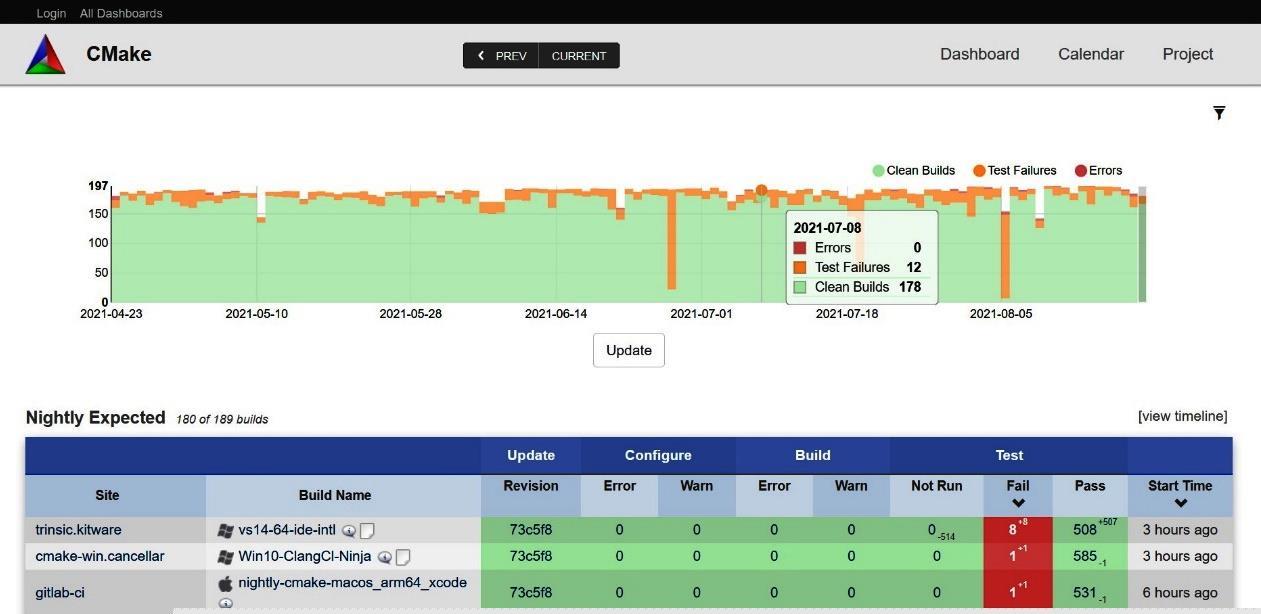
\includegraphics[width=0.8\textwidth]{content/3/chapter8/images/1.jpg}\\
图8.1 CDash仪表板时间轴视图的截图
\end{center}

CDash不在本书的讨论范围内,因为它是作为共享服务器使用的高级解决方案,公司中的所有开发人员都可以访问。

\begin{tcolorbox}[colback=blue!5!white,colframe=blue!75!black,title=Note]
若有兴趣在线学习更多信息,请参考CMake的官方文档并访问CDash的网站:

\url{https://cmake.org/cmake/help/latest/manual/ctest.1.html\#dashboard-client}

\url{https://www.cdash.org/}
\end{tcolorbox}

回到前两种模式。测试模式的命令行如下所示:

\begin{tcblisting}{commandshell={}}
ctest [<options>]
\end{tcblisting}

这种模式下,使用cmake构建项目之后,应该在构建树中执行CTest。这在开发周期中有点麻烦,因为需要执行多个命令并来回更改工作目录。为了简化这个过程,CTest添加了第二个模式:构建-测试模式。

\subsubsubsection{8.3.1\hspace{0.2cm}构建和测试模式}

要使用这种模式,需要执行以-{}-build-and-test开头的ctest,如下所示:

\begin{tcblisting}{commandshell={}}
ctest --build-and-test <path-to-source> <path-to-build>
      --build-generator <generator> [<options>...]
      [--build-options <opts>...]
      [--test-command <command> [<args>...]]
\end{tcblisting}

这是对常规测试模式的简单包装,接受一些构建配置选项,允许为第一种模式附加命令——可以传递给ctest <options>的选项在传递给ctest -{}-build-and-test时都将工作。要求是在-{}-test-command参数后面传递完整的命令。不过,构建-测试模式实际上不会运行任何测试,除非在-{}-testcommand后面提供ctest关键字,如下所示:

\begin{tcblisting}{commandshell={}}
ctest --build-and-test project/source-tree /tmp/build-tree
--build-generator "Unix Makefiles" --test-command ctest
\end{tcblisting}

这个命令中,指定源和构建路径,并选择一个构建生成器。所有这三个都是必须的,并且遵循cmake命令的规则,在第1章中有详细描述。

可以向此模式传递附加参数。分为三组,分别控制配置、构建过程或测试。

以下是控制配置阶段的参数:

\begin{itemize}
\item 
-{}-build-options—cmake配置(不是构建工具)的任何额外选项都应该在-{}-test-command之前提供,-{}-test-command位于最后。

\item 
-{}-build-two-config—为CMake运行两次配置阶段。

\item 
-{}-build-nocmake—跳过配置阶段。

\item 
-{}-build-generator-platform, --build-generator-toolset— 提供生成器特定的平台和工具集。

\item 
-{}-build-makeprogram—当使用基于make或基于ninja的生成器时,需要指定make可执行文件。
\end{itemize}

以下是控制构建阶段的点:

\begin{itemize}
\item 
-{}-build-target—构建指定的目标(而不是所有目标)。
	
\item 
-{}-build-noclean—在不构建干净目标的情况下进行构建。
	
\item 
-{}-build-project—提供所构建项目的名称。
\end{itemize}

用来控制测试阶段的参数:

\begin{itemize}
\item 
-{}-test-timeout—限制测试的执行(以秒为单位)。
\end{itemize}

剩下的就是在-{}-test-command参数之后配置常规测试模式。

\subsubsubsection{8.3.2\hspace{0.2cm}测试模式}

假设已经构建了项目,并且在构建树中执行ctest(或者使用构建-测试包装器),可以执行测试。

大多数情况下,不带参数的简单ctest命令通常就足以获得令人满意的结果。若所有测试都通过,ctest将返回一个0退出代码。在CI/CD流水中使用此功能,以防止错误提交合并到存储库的生产分支。

编写好的测试可能与编写生产代码本身一样具有挑战性。将SUT设置为特定的状态,运行一个测试,然后销毁SUT实例。这个过程相当复杂,可能会产生各种各样的问题:交叉测试污染、时间和并发中断、资源争用、死锁导致的执行停滞,以及许多其他问题。

可以采用有助于发现和解决其中一些问题的策略。CTest允许选择测试、测试顺序、产生的输出、时间限制、重复次数等。以下各节将提供必要的背景和对最有用的选项的简要概述,请参阅CMake文档以获得详尽的列表。

\hspace*{\fill} \\ %插入空行
\noindent
\textbf{查询测试}

可能需要做的第一件事是了解哪些测试实际上是为项目编写的。CTest提供了一个-N选项,其禁用执行,只打印一个列表,如下所示:

\begin{tcblisting}{commandshell={}}
# ctest -N
Test project /tmp/b
  Test #1: SumAddsTwoInts
  Test #2: MultiplyMultipliesTwoInts
Total Tests: 2
\end{tcblisting}

可能希望在下一节中描述的筛选器中使用-N,以检查在应用筛选器时将执行哪些测试。

若需要一个可以自动化工具使用的JSON格式,请使用-{}-show-only=json-v1执行ctest。

CTest还提供了一种用LABELS关键字对测试进行分组的机制。要列出所有可用的标签(而不实际执行任何测试),请使用-{}-print-labels。当在列表文件中使用add\_test(<name> <testcommand>)指令手动定义测试时,这个选项很有用,可以通过测试属性指定单独的标签:

\begin{lstlisting}[style=styleCMake]
set_tests_properties(<name> PROPERTIES LABELS "<label>")
\end{lstlisting} 

另一方面,稍后将讨论的框架提供自动测试发现,但它还不支持这种细粒度级别的标记。

\hspace*{\fill} \\ %插入空行
\noindent
\textbf{过滤测试}

有很多理由只运行所有测试的一个子集——最常见的原因可能是需要调试单个失败的测试或正在处理的模块。这种情况下,没有必要等待所有其他测试。其他高级的测试场景甚至可以划分测试用例,并将负载分布到测试运行人员的团队中。

这些标志将根据提供的<r>正则表达式(正则表达式)筛选测试,如下所示:

\begin{itemize}
\item 
-R <r>, -{}-tests-regex <r>—只运行名称匹配<r>的测试

\item 
-E <r>, -{}-exclude-regex <r>—跳过名称匹配<r>的测试

\item 
-L <r>, -{}-label-regex <r>—只运行标签匹配<r>的测试

\item 
-LE <r>, -{}-label-exclude <regex>—跳过标签匹配<r>的测试
\end{itemize}

高级场景可以通过-{}-tests-information选项(或缩写形式-i)实现。使用此过滤器以逗号分隔的格式提供一个范围:<start>,<end>,<step>。任何字段都可以为空,在多一个逗号之后,可以附加单个<test-id>值以额外运行它们。下面是一些例子:

\begin{itemize}
\item 
-I 3,, 将跳过测试1和2(从第三个测试开始执行)

\item 
-I ,2, 只运行第一个和第二个测试

\item 
-I 2,,3 从一行中的第二个测试开始,每隔第三个测试运行一次

\item 
-I ,0,,3,9,7 只运行第三、第九和第七个测试
\end{itemize}

CTest可以选择接受包含相同格式的规范的文件名,用户更喜欢按名称筛选测试。此选项可用于为非常大的套件在多台机器上分发测试。

默认情况下,与-R一起使用的-I选项将缩小执行范围(只有同时满足两个需求的测试才会运行)。若需要执行两者的并集(需求都可以满足),则添加-U选项。

如前所述,可以使用-N选项检查过滤的结果。

\hspace*{\fill} \\ %插入空行
\noindent
\textbf{乱序测试}

编写单元测试可能很棘手。遇到的一个更令人惊讶的问题是测试耦合,即一个测试通过不完全设置,或清除SUT状态而影响另一个测试的情况。换句话说,要执行的第一个测试可能“泄漏”状态并污染第二个测试。这样的耦合是坏消息,因为这引入了测试之间未知的隐式关系。

更糟糕的是,这种错误可以很好地隐藏在复杂的测试场景中。将导致一个测试在不应该的情况下失败时,可能会检测到它,但相反的情况也同样可能发生:不正确的状态导致测试在不应该的情况下通过。这种错误地通过测试给了开发人员一种安全的错觉,这甚至比根本不进行测试还要糟糕。对代码进行了正确测试的假设可能会鼓励更大胆的行动,导致意想不到的结果。

发现此类问题的一种方法是单独运行每个测试。通常,在没有CTest的情况下直接从测试框架执行测试运行程序时,情况就不是这样了。要运行单个测试,您需要向测试可执行文件传递一个特定于框架的参数。这允许检测在套件中通过,但在单独执行时失败的测试。

另一方面,CTest通过隐式执行子CTest实例中的每个测试用例,有效地消除了所有基于内存的测试交叉污染。甚至可以进一步添加-{}-force-new-ctest-process选项来强制单独的进程。

但当测试正在使用外部的、有争议的资源(如GPU、数据库或文件),那么仅靠这一点是不起作用的。可以采取的另一个预防措施,简单地随机化测试执行的顺序。这种干扰往往足以最终检测出这种虚假通过的测试。CTest通 -{}-schedulerandom选项支持这种策略。

\hspace*{\fill} \\ %插入空行
\noindent
\textbf{处理失败}

John C. Maxwell有句名言:“尽早失败,经常失败,但总是向前失败。”这正是在运行单元测试时想要做的事情(也许在生活的其他领域也是如此)。除非在运行带有调试器的测试时,否则不容易了解在哪里犯了错误,因为CTest将保持内容简短,只列出失败的测试,而不实际打印任何输出。

由测试用例或SUT打印到标准输出的消息对于确定错误的确切位置可能非常有用。要查看它们,可以运行ctest with -{}-output-on-failure。或者,设置CTEST\_OUTPUT\_ON\_FAILURE环境变量也会有相同的效果。

根据解决方案的大小,在测试失败后停止执行可能是有意义的。可以通过-{}-stop-on-failure参数来实现。

CTest存储失败测试的名称。为了在冗长的测试套件中节省时间,可以将重点放在这些失败的测试上,并在问题解决之前跳过运行通过的测试。

该特性是通过-{}-rerun-failed选项启用的(其他过滤器都将忽略)。记住在解决所有问题后运行所有测试,以确保在此期间没有引入回归。

当CTest没有检测到测试时,这可能意味着两件事:要么没有测试,要么项目有问题。默认情况下,ctest将打印一条警告消息并返回一个0退出代码,以避免混淆视听。大多数用户将有足够的上下文来理解他们遇到的情况和下一步要做什么。然而,某些环境中,ctest将始终作为自动化流水的一部分执行。

然后,可能需要显式地表示,缺乏测试应该解释为错误(并返回非零退出码)。可以通过提供-{}-no-tests=error参数来配置这种行为。对于相反的行为(没有警告),使用-{}-no-tests=ignore选项。

\hspace*{\fill} \\ %插入空行
\noindent
\textbf{重复测试}

在职业生涯中,迟早会遇到大多数时候都能正常工作的测试。这些测试极有可能因为环境原因而失败:错误的模拟时间、事件循环问题、异步执行的糟糕处理、并行性、哈希冲突,以及其他并非每次运行都发生的非常复杂的场景。这些不可靠的测试被称为“片状测试”。

这种不一致似乎不是一个重要的问题,测试不是真正的生产环境,这是它们有时失败的最终原因。有一点是正确的:测试并不意味着复制每一个小细节,因为是不可行的。测试是一种模拟,对可能发生的情况的近似,这通常就足够了。若测试在下次执行时会通过,那么重新运行测试是否会造成伤害?

事实上,确实如此。这里概述了三个主要问题:

\begin{itemize}
\item 
若代码库中收集了足够多的零散测试,将成为代码更改顺利交付的严重障碍。当赶时间的时候,尤其令人沮丧:要么是在周五下午准备回家,要么是在为影响客户的严重问题进行关键修复。

\item 
不能确定,是否由于测试环境的不适当,不可靠的测试正在失败。事实可能恰恰相反:它们失败是因为复制了生产中已经出现的罕见场景。只是还没有明显到可以拉响警报的程度。

\item 
不是测试有问题,而是代码有问题!环境有时是不稳定的,作为开发者,需要以确定的方式处理它。若SUT以这种方式运行,这是一个严重的错误——例如,代码可能正在从未初始化的内存中读取。
\end{itemize}

没有一种完美的方法可以解决上述所有情况——可能的原因太多了。但可以通过-repeat <mode>:<\#>选项反复运行测试,从而增加识别不可靠测试的机会。有三种模式可供选择,如下所述:

\begin{itemize}
\item 
until-fail—运行测试<\#>次;所有的测试都必须通过。

\item 
until-pass—运行测试到<\#>次;至少要通过一次。这在处理已知的不稳定、但太难调试或不能禁用的测试时非常有用。

\item 
after-timeout—运行测试直到<\#>次,但只有在测试超时时才重试。可以在负载过高的测试环境中使用。
\end{itemize}

一般的建议是尽可能快地调试不可靠的测试,若不能相信它们能产生一致的结果,就去掉它们。

\hspace*{\fill} \\ %插入空行
\noindent
\textbf{控制输出}

每次将信息打印到屏幕上都会立刻变得异常繁忙。CTest减少噪音并收集它执行到日志文件的测试的输出,只提供关于常规运行的最有用的信息。当情况变糟,测试失败时,若启用了-{}-output-onfailure,就可以预期得到一个摘要和一些日志。

从经验中知道,“足够的信息”是足够的。但有时,可能也想查看通过的测试的输出,也许是为了检查它们是否真的在工作(而不是没有错误地默默地停止)。要访问更详细的输出,添加-v选项(或者-{}-verbose,若想在自动化流水中显式显示)。

若这还不够,可能需要-VV或-{}-extra-verbose。对于非常深入的调试,请使用-{}-debug(但要准备好面对包含所有细节的文本墙)。若想要的是相反的,CTest还提供“禅模式”,启用-q或-{}-quiet。没有输出将打印出来(可以停止担心,学会享受平静)。这个选项似乎除了迷惑人们之外没有其他用途,但是要注意输出仍然会存储在测试文件中(默认情况下在./Testing/Temporary中)。自动化流水可以检查退出代码是否为非零值,并收集日志文件以进行进一步处理,而不会用可能使不熟悉产品的开发人员感到困惑的信息(从而破坏主要输出)。

使用-O <file>,-{}-output-log <file>选项将日志存储在指定的路径中。若遇到了冗长的输出,可以使用两个限制选项来限制每个测试的给定字节数:-{}-test-output-size-passed <size>和-{}-test-output-size-failed <size>。

\hspace*{\fill} \\ %插入空行
\noindent
\textbf{其他选项}

对于日常测试需求,还有其他一些有用的选项:

\begin{itemize}
\item 
-C <cfg>, -{}-build-config <cfg> (仅支持多配置生成器)——指定要测试的配置。Debug配置通常有调试符号,但是Release也应该进行测试,因为大量的优化选项可能会潜在地影响SUT的行为。

\item 
-j <jobs>, -{}-parallel <jobs>—这将设置并行执行的测试数。这对于在开发过程中加速长时间测试的执行非常有用。注意,在繁忙的环境中(在共享测试运行器上),可能会由于调度而产生不利影响。下一个选项可以稍微缓解这种情况

\item 
-{}-test-load <level>—使用此选项调度并行测试,使CPU负载不超过<level>值(在尽最大努力的基础上)。

\item 
-{}-timeout <seconds>—使用此命令指定单个测试的默认时间限制。
\end{itemize}

现在已经了解了如何在许多不同的场景中执行ctest。接下来,让我们学习如何添加一个测试。


























